% Compiling with
% latexmk -halt-on-error -shell-escape -synctex=1 -pdf
% (Recommend using a latexmkrc file so as just to run latexmk -pvc, for example)
% Probably you can achieve the same with an inordinate number of invocations of
% pdflatex -halt-on-error -shell-escape -synctex=1

% fleqn aligns equations to the left, a4 paper size, 11pt font, article class
\documentclass[fleqn,a4paper,11pt]{article}
\title{IA Vectors and Matrices Example Sheet 4 (revised)}
\author{Izaak van Dongen (\texttt{imv26})}

\usepackage{mymaths}
\usepackage{mystyle}

\begin{document}
 \maketitle\thispagestyle{empty} % no page number under title

 \begin{enumerate}[label=\textbf{\arabic*.}]
  \item
   If \(\mat A\) is an \(n \times n\) upper triangular matrix, we can calculate
   \begin{align*}
    \chi_{\mat A}(t)
     &= \det(\mat A - t \mat I) \\
     &=
      \begin{vmatrix}
       A_{11} - t & A_{12} & A_{13} & \dotsm \\
       0 & A_{22} - t & A_{23} & \dotsm \\
       0 & 0 & A_{33} - t & \dotsm \\
       \vdots & \vdots & \vdots & \ddots
      \end{vmatrix} \\
     &=
      (A_{11} - t)
      \begin{vmatrix}
       A_{22} - t & A_{23} & \dotsm \\
       0 & A_{33} - t & \dotsm \\
       \vdots & \vdots & \ddots
      \end{vmatrix} \quad \text{by expanding along the first column} \\
     &= (A_{11} - t)(A_{22} - t) \dotsm (A_{nn} - t)
      \quad \text{by induction on \(n\)}
   \end{align*}
   So clearly the roots of \(\chi_{\mat A}(t)\) (ie the eigenvalues of
   \(\mat A\)) are precisely \(A_{11}, \dotsc, A_{nn}\).
  \item \(
   \begin{aligned}[t]
    \chi_{\mat M}(t)
     &= \det(\mat M - t \mat I) \\
     &=
     \begin{vmatrix}
      -t & 1 & 0 \\
      -4 & 4 - t & 0 \\
      -2 & 1 & 2 - t
     \end{vmatrix} \\
     &= -t(4 - t)(2 - t) - 1(-4)(2 - t) \\
     &= (2 - t)( -t(4 - t) + 4) \\
     &= (2 - t)(t^2 - 4t + 4) \\
     &= (2 - t)^3
   \end{aligned} \)

   so \(\mat M\) has characteristic equation
   \((2 - t)^3 = 0 \iff (t - 2)^3 = 0\).

   In order for \(\mat M\) to be diagonalisable its single eigenvalue would have
   to have geometric multiplicity \(3\), which would imply that the eigenspace
   of the eigenvalue \(2\) is all of \(\Reals^3\). This is clearly not the
   case, since \(\mat M \vec e_1 \ne 2\vec e_1\).
  \item
   The orthogonality of this matrix is precisely equivalent to the
   orthonormality of its columns. Since the first two columns are orthonormal
   (by checking \(\frac 19 + \frac 49 + \frac 49 = 1\),
   \(\frac 12 + \frac 12 = 1\) and
   \(\frac 12 \sqrt 2(\frac 23 - \frac 23) = 0\)), we need the third column to
   be orthogonal to both, and have unit length. There are two such vectors -
   \((\frac 13, \frac 23, \frac 23) \veccross \sqrt 2(0, \frac 12, \frac 12)
     = (-\frac 23 \sqrt 2, \frac 16 \sqrt 2, \frac 16 \sqrt 2)\)
   and \(-1\) times the above, so \(a, b, c\) are only uniquely determined up to
   sign.
  \item
   It has characteristic equation
   \begin{align*}
    \chi_{\mat A}
     &= \det{\mat A - t \mat I} \\
     &=
     \begin{vmatrix}
      3 - t & 1 & 1 \\
      1 & 2 - t & 0 \\
      1 & 0 & 2 - t
     \end{vmatrix} \\
    &= (3 - t)(2 - t)(2 - t) - (2 - t) - (2 - t) \\
    &= (2 - t)[(3 - t)(2 - t) - 2] \\
    &= (2 - t)(t^2 - 5t + 4) \\
    &= (2 - t)(t - 4)(t - 1)
   \end{align*}
   so the eigenvalues of \(\mat A\) are \(1, 2, 4\). We can then calculate its
   eigenvectors, and we know each has geometric multiplicity \(1\) since we have
   three distinct.
   \begin{alignat*}3
    \lambda_1 = 1:\quad{}&& &&
    \begin{pmatrix}
     2 & 1 & 1 \\
     1 & 1 & 0 \\
     1 & 0 & 1
    \end{pmatrix}
    \vec v_1 &= \vec 0 \\
    \parens{
     \vec r(1) \to \vec r(1) - \vec r(2) - \vec r(3)
    }\quad
    &&\iff{}&&
    \begin{pmatrix}
     0 & 0 & 0 \\
     1 & 1 & 0 \\
     1 & 0 & 1
    \end{pmatrix}
    \vec v_1 &= \vec 0 \\
    &&\impliedby{}&&
    \vec v_1 &= \begin{pmatrix*}[r] 1 \\ -1 \\ -1 \end{pmatrix*} \\
    \lambda_2 = 2:\quad{}&& &&
    \begin{pmatrix}
     1 & 1 & 1 \\
     1 & 0 & 0 \\
     1 & 0 & 0
    \end{pmatrix}
    \vec v_2 &= \vec 0 \\
    &&\impliedby{}&&
    \vec v_2 &= \begin{pmatrix*}[r] 0 \\ 1 \\ -1 \end{pmatrix*} \\
    \lambda_3 = 4:\quad{}&& &&
    \begin{pmatrix*}[r]
     -1 & 1 & 1 \\
     1 & -2 & 0 \\
     1 & 0 & -2
    \end{pmatrix*}
    \vec v_3 &= \vec 0 \\
    \parens{
     \vec r(1) \to \vec r(1) + \tfrac 12\vec r(2) + \tfrac 12\vec r(3)
    }\quad
    &&\iff{}&&
    \begin{pmatrix*}[r]
     0 & 0 & 0 \\
     1 & -2 & 0 \\
     1 & 0 & -2
    \end{pmatrix*}
    \vec v_3 &= \vec 0 \\
    &&\impliedby{}&&
    \vec v_3 &= \begin{pmatrix} 2 \\ 1 \\ 1 \end{pmatrix}
   \end{alignat*}
   Noting that these are orthogonal, we can normalise each eigenvector to get an
   orthonormal set. Hence \(\tran{\mat P} \mat A \mat P = \mat D\), where
   \begin{equation*}
    \mat P =
    \begin{pmatrix*}[r]
     \frac 13 \sqrt 3  & 0                 & \frac 13 \sqrt 6 \\[0.5ex]
     -\frac 13 \sqrt 3 & \frac 12 \sqrt 2  & \frac 16 \sqrt 6 \\[0.5ex]
     -\frac 13 \sqrt 3 & -\frac 12 \sqrt 2 & \frac 16 \sqrt 6
    \end{pmatrix*}, \quad
    \mat D =
    \begin{pmatrix}
     1 & 0 & 0 \\
     0 & 2 & 0 \\
     0 & 0 & 4
    \end{pmatrix}
   \end{equation*}
   (so \(\mat P \tran{\mat P} = \mat I\)) and hence
   \begin{align*}
    \mat A^{-1}
    &= \mat P \mat D^{-1} \tran{\mat P} \\
    &=
    \begin{pmatrix*}[r]
     \frac 13 \sqrt 3  & 0                 & \frac 13 \sqrt 6 \\[0.5ex]
     -\frac 13 \sqrt 3 & \frac 12 \sqrt 2  & \frac 16 \sqrt 6 \\[0.5ex]
     -\frac 13 \sqrt 3 & -\frac 12 \sqrt 2 & \frac 16 \sqrt 6 \\[0.5ex]
    \end{pmatrix*}
    \begin{pmatrix}
     1 & 0 & 0 \\
     0 & \frac 12 & 0 \\
     0 & 0 & \frac 14
    \end{pmatrix}
    \begin{pmatrix*}[r]
     \frac 13 \sqrt 3  & -\frac 13 \sqrt 3 & -\frac 13 \sqrt 3 \\[0.5ex]
     0 & \frac 12 \sqrt 2 & -\frac 12 \sqrt 2 \\[0.5ex]
     \frac 13 \sqrt 6 & \frac 16 \sqrt 6 & \frac 16 \sqrt 6 \\[0.5ex]
    \end{pmatrix*} \\
    &=
    \begin{pmatrix*}[r]
     \frac 13 \sqrt 3  & 0                 & \frac 13 \sqrt 6 \\[0.5ex]
     -\frac 13 \sqrt 3 & \frac 12 \sqrt 2  & \frac 16 \sqrt 6 \\[0.5ex]
     -\frac 13 \sqrt 3 & -\frac 12 \sqrt 2 & \frac 16 \sqrt 6 \\[0.5ex]
    \end{pmatrix*}
    \begin{pmatrix*}[r]
     \frac 13 \sqrt 3  & -\frac 13 \sqrt 3 & -\frac 13 \sqrt 3 \\[0.5ex]
     0 & \frac 14 \sqrt 2 & -\frac 14 \sqrt 2 \\[0.5ex]
     \frac 1{12} \sqrt 6 & \frac 1{24} \sqrt 6 & \frac 1{24} \sqrt 6 \\[0.5ex]
    \end{pmatrix*} \\
    &=
    \begin{pmatrix}
     \frac 13 + \frac 16
      & -\frac 13 + \frac 1{12}
      & -\frac 13 + \frac 1{12} \\[0.5ex]
     -\frac 13 + \frac 1{12}
      & \frac 13 + \frac 14 + \frac 1{24}
      & \frac 13 - \frac 14 + \frac 1{24} \\[0.5ex]
     -\frac 13 + \frac 1{12}
      & \frac 13 - \frac 14 + \frac 1{24}
      & \frac 13 + \frac 14 + \frac 1{24} \\[0.5ex]
    \end{pmatrix} \\
    &=
    \begin{pmatrix*}[r]
     \frac 12 & -\frac 14 & -\frac 14 \\[0.5ex]
     -\frac 14 & \frac 58 & \frac 18 \\[0.5ex]
     -\frac 14 & \frac 18 & \frac 58 \\[0.5ex]
    \end{pmatrix*}
   \end{align*}
  \item
   This quadratic form is the same as
   \(\mathcal F(\vec x) = \tran{\vec x} \mat A \vec x\)
   where
   \begin{equation*}
    \mat A =
    \begin{pmatrix}
     \alpha & \beta \\
     \beta & \gamma
    \end{pmatrix}
   \end{equation*}
   where \(\alpha = a\cos^2 \theta + b\sin^2 \theta\),
   \(\gamma = a\sin^2 \theta + b\cos^2 \theta\), and
   \(\beta = (a - b)\sin \theta \cos \theta\).
   Then its characteristic polynomial is
   \begin{align*}
    \chi_{\mat A}(t)
    &= \det(\mat A - t\mat I) \\
    &=
    \begin{vmatrix}
     \alpha - t & \beta \\
     \beta & \gamma - t
    \end{vmatrix} \\
    &= (\alpha - t)(\gamma - t) - \beta^2 \\
    &= \alpha \gamma - \beta^2 - (\alpha + \gamma)t + t^2 \\
    &= (a^2 + b^2)\cos^2 \theta \sin^2 \theta
     + ab(\sin^4 \theta + \cos^4 \theta)
     - (a^2 + b^2 - 2ab)\cos^2 \theta \sin^2 \theta
     - (a + b)t + t^2 \\
    &= ab(\sin^4 \theta + 2\cos^2 \theta \sin^2 \theta + \cos^4 \theta)
     - (a + b)t + t^2 \\
    &= ab(\sin^2 \theta + \cos^2 \theta)^2
     - (a + b)t + t^2 \\
    &= ab - (a + b)t + t^2 \\
    &= (a - t)(b - t)
   \end{align*}
   so \(\mat A\) has eigenvalues \(a, b\). Then we can find some unit
   eigenvectors:
   \begin{alignat*}3
    \lambda_1 = a:\quad&& &&
    \begin{pmatrix}
     a \cos^2 \theta + b \sin^2 \theta - a & (a - b)\sin \theta \cos \theta \\
     (a - b) \sin \theta \cos \theta & a \sin^2 \theta + b \cos^2 \theta - a
    \end{pmatrix}
    \vec v_1 &= \vec 0 \\
    &&\iff{}&&
    \begin{pmatrix}
     (b - a)\sin^2 \theta & (a - b)\sin \theta \cos \theta \\
     (a - b) \sin \theta \cos \theta & (b - a)\cos^2 \theta
    \end{pmatrix}
    \vec v_1 &= \vec 0 \\
    &&\impliedby{}&&
    \vec v_1 &= \begin{pmatrix} \cos \theta \\ \sin \theta \end{pmatrix} \\
    \lambda_2 = b:\quad&& &&
    \begin{pmatrix}
     a \cos^2 \theta + b \sin^2 \theta - b & (a - b)\sin \theta \cos \theta \\
     (a - b) \sin \theta \cos \theta & a \sin^2 \theta + b \cos^2 \theta - b
    \end{pmatrix}
    \vec v_2 &= \vec 0 \\
    &&\iff{}&&
    \begin{pmatrix}
     (a - b) \cos^2 \theta & (a - b)\sin \theta \cos \theta \\
     (a - b) \sin \theta \cos \theta & (a - b) \sin^2 \theta
    \end{pmatrix}
    \vec v_2 &= \vec 0 \\
    &&\impliedby{}&&
    \vec v_2 &= \begin{pmatrix} -\sin \theta \\ \cos \theta \end{pmatrix}
   \end{alignat*}
   so its principal axes are along \(\vec v_1\) and \(\vec v_2\) with
   eigenvalues \(a\) and \(b\) respectively. It could be written
   \(au^2 + bv^2\) where
   \(u = \vec x \vecdot \vec v_1 = x \cos \theta + y \sin \theta\) and
   \(v = \vec x \vecdot \vec v_2 = -x \sin \theta + y \cos \theta\) are the
   components along these axes.
  \item
   \begin{enumerate}[label=(\roman*)]
    \item
     Let \(\lambda\) be an arbitrary eigenvalue of \(\mat A\). Then there is
     some nonzero eigenvector \(\vec v\) such that
     \(\mat A \vec v = \lambda \vec v\). Taking the inner product with
     \(\vec v\), we get
     \begin{alignat*}2
      && \herm{(\mat A \vec v)} \vec v
      &= \herm{(\lambda \vec v)} \vec v \\
      \implies{}&&
      \herm{\vec v} \herm{\mat A} \vec v
      &= \conj \lambda \herm{\vec v} \vec v \\
      \implies{}&&
      \herm{\vec v} (-\mat A \vec v)
      &= \conj \lambda \herm{\vec v} \vec v \\
      \implies{}&&
      -\lambda \herm{\vec v} \vec v
      &= \conj \lambda \herm{\vec v} \vec v
     \end{alignat*}
     so \(-\lambda = \conj \lambda\), since \(\vec v \ne \vec 0\), and hence
     \(\Re(\lambda) = \frac 12(\lambda + \conj \lambda) = 0\), so \(\lambda\)
     is purely imaginary.

     Furthermore, if there are two eigenvectors \(\vec v_1, \vec v_2\)
     associated with distinct eigenvalues \(\lambda_1, \lambda_2\), then
     consider
     \begin{align*}
      -\lambda_1 \herm{\vec v_1} \vec v_2
      &= \conj{\lambda_1} \herm{\vec v_1} \vec v_2 \\
      &= \herm{(\lambda_1 \vec v_1)} \vec v_2 \\
      &= \herm{(\mat A \vec v_1)} \vec v_2 \\
      &= \herm{\vec v_1} \herm{\mat  A} \vec v_2 \\
      &= -\herm{\vec v_1} \mat  A \vec v_2 \\
      &= -\lambda_2 \herm{\vec v_1} \vec v_2
     \end{align*}
     and since \(-\lambda_1 \ne -\lambda_2\), \(\herm{\vec v_1}\vec v_2 = 0\),
     ie \(\vec v_1\) and \(\vec v_2\) are orthogonal.
    \item
     Let \(\lambda\) be an arbitrary eigenvalue of \(\mat U\). Then there is
     some nonzero eigenvector \(\vec v\) such that
     \(\mat U \vec v = \lambda \vec v\). Taking norms on both sides, we get
     \begin{alignat*}2
      && \herm{(\mat U \vec v)} \mat U \vec v
      &= \herm{(\lambda \vec v)} \lambda \vec v \\
      \implies{}&&
      \herm{\vec v} \herm{\mat U} \mat U \vec v
      &= \conj \lambda \lambda \herm{\vec v} \vec v \\
      \implies{}&&
      \herm{\vec v} \vec v
      &= \abs{\lambda}^2 \herm{\vec v} \vec v \\
      \implies{}&&
      \abs{\lambda}^2 &= 1 \\
      \implies{}&&
      \abs{\lambda} &= 1
     \end{alignat*}
     Furthermore, if there are two eigenvectors \(\vec v_1, \vec v_2\)
     associated with distinct eigenvalues \(\lambda_1, \lambda_2\), then
     consider
     \begin{align*}
      \herm{\vec v_1} \vec v_2
      &= \herm{\vec v_1} \herm{\mat U} \mat U \vec v_2 \\
      &= \herm{(\mat U \vec v_1)} \mat U \vec v_2 \\
      &= \herm{(\lambda_1 \vec v_1)} (\lambda_2 \vec v_2) \\
      &= \conj{\lambda_1} \lambda_2 \herm{\vec v_1} \vec v_2
     \end{align*}
     but
     \(\conj{\lambda_1} \lambda_2 = 1 \iff \lambda_1 = \lambda_2\), since both
     have modulus \(1\) and the multiplicative inverse of \(\lambda_2\) is
     \(\conj{\lambda_2}\). Therefore again \(\herm{\vec v_1} \vec v_2 = 0\) and
     the eigenvectors are orthogonal.
   \end{enumerate}
  \item
   Let \(\mat M = \begin{psmallmatrix} a & b \\ c & d \end{psmallmatrix}\) be an
   arbitrary \(2 \times 2\) matrix. Then we can calculate
  \begin{align*}
   \chi_{\mat M}(t)
   &= \det(\mat M - t \mat I) \\
   &=
   \begin{vmatrix}
    a - t & b \\
    c & d - t
   \end{vmatrix} \\
   &= (a - t)(d - t) - bc \\
   &= t^2 - (a + d)t + ad - bc
  \end{align*}
  and verify that
  \begin{align*}
   \text{``\(\chi_{\mat M}(\mat M)\)''}
   &= \mat M^2 - (a + d)\mat M + (ad - bc)\mat I \\
   &=
   \begin{pmatrix}
    a & b \\
    c & d
   \end{pmatrix}^2
   - (a + d)\begin{pmatrix}
    a & b \\
    c & d
   \end{pmatrix}
   + (ad - bc)\begin{pmatrix}
    1 & 0 \\
    0 & 1
   \end{pmatrix} \\
   &=
   \begin{pmatrix}
    a^2 + bc & ab + bd \\
    ac + cd & bc + d^2
   \end{pmatrix}
   - \begin{pmatrix}
    a^2 + ad & ab + bd \\
    ac + cd & ad + d^2
   \end{pmatrix}
   + \begin{pmatrix}
    ad - bc & 0 \\
    0 & ad - bc
   \end{pmatrix} \\
   &= \mat 0
  \end{align*}
  Now
  \begin{align*}
   \chi_{\mat A}(t)
   &= \det(\mat A - t\mat I) \\
   &=
   \begin{vmatrix}
    3 - t & 4 \\
    -1 & -1 - t
   \end{vmatrix} \\
   &= (t - 3)(t + 1) + 4 \\
   &= t^2 - 2t + 1
  \end{align*}
  and hence
  \(\mat A^2 - 2\mat A + \mat I = \mat 0 \implies
    \mat A^2 = 2\mat A - \mat I\) as required.
  \(\mat A\) also only has a single eigenvalue \(\lambda = 1\), with algebraic
  multiplicity \(2\). In finding its eigenspace, we see that
  \begin{alignat*}3
   && &&
   \begin{pmatrix}
    2 & 4 \\
    -1 & -2
   \end{pmatrix}
   \vec v &= \vec 0 \\
   \parens*{
    \begin{aligned}
     \vec r(1) &\to \vec r(1) + 2 \vec r(2) \\
     \vec r(2) &\to -\vec r(2)
    \end{aligned}
   }&& \iff{}&&
   \begin{pmatrix}
    0 & 0 \\
    1 & 2
   \end{pmatrix}
   \vec v &= \vec 0 \\
   && \iff{}&&
   \begin{pmatrix} 1 \\ 2 \end{pmatrix} \vecdot \vec v &= \vec 0
  \end{alignat*}
  which is a line, which is to say this eigenvalue has geometric multiplicity
  \(1\) and \(\mat A\) does not give rise to an eigenbasis for \(\Reals^2\), so
  \(\mat A\) is not diagonalisable.

  The cases \(n = 0, 1\) are trivial, and the case \(n = 2\) was demonstrated
  above. In general,
  \begin{align*}
   \mat A^{n + 1}
   &= \mat A \mat A^n \\
   &= \mat A (\alpha_n \mat A + \beta_n \mat I) \quad
      \text{by inductive hypothesis} \\
   &= \alpha_n \mat A^2 + \beta_n \mat A \\
   &= \alpha_n (2\mat A - \mat I) + \beta_n \mat A \\
   &= (2\alpha_n + \beta_n)\mat A - \alpha_n \mat I
  \end{align*}
  giving rise to the recurrence relations
  \(\alpha_{n + 1} = 2 \alpha_n + \beta_n\) and \(\beta_{n + 1} = -\alpha_n\),
  with initial conditions
  \(\alpha_0 = 0\), \(\beta_0 = 1\), (\(\alpha_1 = 1\), \(\beta_1 = 0\))

  Then it's easiest to just spot by trying some numbers that this induces a nice
  pattern on \(\alpha_n\) and \(\beta_n\) - particularly,
  \(\alpha_n = n\) and \(\beta_n = 1 - n\). We can check that these suit the
  initial conditions and that indeed we have
  \(\alpha_{n + 1} = 2\alpha_n + \beta_n = 2n + (1 - n) = n + 1\) and
  \(\beta_{n + 1} = -\alpha_n = -n = 1 - (1 + n)\).

  So, explicitly, \(\mat A^n = n\mat A + (1 - n)\mat I\).
 \item
  The matrix \(\mat A\) is such that for each \(i = 1, \dotsc, n\),
  \(T(\vec e_i) = \vec f_j A_{ji}\). That is, the \(i\)th column of \(\mat A\)
  is the coefficents representing the image of \(\vec e_i\) under \(T\) in the
  \(\set{\vec f_1, \dotsc, \vec f_m}\) basis.
  \begin{enumerate}[label=(\alph*)]
   \item
    Here \(T\) is represented by the matrix
    \begin{equation*}
     \mat A =
     \begin{pmatrix}
      2 & 7 \\
      1 & 0 \\
      5 & 3
     \end{pmatrix}
    \end{equation*}
    in the standard basis, and will be represented by
    \begin{equation*}
     \mat A' =
     \begin{pmatrix}
      1 & 0 & 0 \\
      0 & 1 & 0 \\
      0 & 0 & 1
     \end{pmatrix}^{-1}
     \begin{pmatrix}
      2 & 7 \\
      1 & 0 \\
      5 & 3
     \end{pmatrix}
     \begin{pmatrix*}[r]
      1 & -3 \\
      -1 & 2
     \end{pmatrix*}
     =
     \begin{pmatrix}
      2 - 7 & -6 + 14 \\
      1 - 0 & -3 + 0 \\
      5 - 3 & -15 + 6
     \end{pmatrix}
     =
     \begin{pmatrix*}[r]
      -5 & 8 \\
      1 & -3 \\
      2 & -9
     \end{pmatrix*}
    \end{equation*}
    in the new basis.
   \item
    This is also known as the plane
    \begin{equation*}
     \begin{pmatrix} \sin \theta \\ -\cos \theta \\ 0 \end{pmatrix}
      \vecdot \vec x = 0
    \end{equation*}
    so a convenient choice of basis is one with two vectors in the plane and one
    normal to the plane - for example, let
    \begin{equation*}
     \vec e_1 = \begin{pmatrix} \sin \theta \\ -\cos \theta \\ 0 \end{pmatrix},
     \quad
     \vec e_2 = \begin{pmatrix} \cos \theta \\ \sin \theta \\ 0 \end{pmatrix},
     \quad
     \vec e_3 = \begin{pmatrix} 0 \\ 0 \\ 1 \end{pmatrix}
    \end{equation*}
    and then the reflection \(T\) is just scaling the coordinate in the axis
    normal to the plane by \(-1\):
    \begin{equation*}
     \mat A =
     \begin{pmatrix*}[r]
      -1 & 0 & 0 \\
      0 & 1 & 0 \\
      0 & 0 & 1
     \end{pmatrix*}
    \end{equation*}
   \item
    In the standard basis,
    \begin{equation*}
     \mat A =
     \begin{pmatrix}
      1 & \lambda \\
      0 & 1
     \end{pmatrix}
    \end{equation*}
    In the new basis,
    \begin{equation*}
     \vec e_1' = \vec f_1' = \begin{pmatrix*}[r] 0 \\ -1 \end{pmatrix*}, \quad
     \vec e_2' = \vec f_2' = \begin{pmatrix} 1 \\ 0 \end{pmatrix}
    \end{equation*}
    so
    \begin{align*}
     \mat A'
     &=
     \begin{pmatrix*}[r]
      0 & 1 \\
      -1 & 0
     \end{pmatrix*}^{-1}
     \begin{pmatrix}
      1 & \lambda \\
      0 & 1
     \end{pmatrix}
     \begin{pmatrix*}[r]
      0 & 1 \\
      -1 & 0
     \end{pmatrix*} \\
     &=
     \begin{pmatrix*}[r]
      0 & -1 \\
      1 & 0
     \end{pmatrix*}
     \begin{pmatrix}
      -\lambda & 1 \\
      -1 & 0
     \end{pmatrix} \\
     &=
     \begin{pmatrix*}[r]
      1 & 0 \\
      -\lambda & 1
     \end{pmatrix*}
    \end{align*}
    The very first line above shows that
    \(\mat A' = \mat R^{-1} \mat A \mat R\) where
    the change-of-basis matrix is the rotation matrix
    \(\mat R = \begin{psmallmatrix*}[r] 0 & 1 \\ -1 & 0 \end{psmallmatrix*}\) -
    a clockwise rotation by \(\degrees{90}\).

    This is really just a consequence of the fact that this basis is produced
    from the standard basis by this rotation.
  \end{enumerate}
 \item
  Here
  \begin{align*}
   \mat B
   &=
   \begin{pmatrix}
    3 & 1 \\
    2 & 1
   \end{pmatrix}^{-1}
   \begin{pmatrix}
    -5 & 9 \\
    -4 & 7
   \end{pmatrix}
   \begin{pmatrix}
    3 & 1 \\
    2 & 1
   \end{pmatrix} \\
   &=
   \begin{pmatrix*}[r]
    1 & -1 \\
    -2 & 3
   \end{pmatrix*}
   \begin{pmatrix}
   -15 + 18 & -5 + 9 \\
   -12 + 14 & -4 + 7
   \end{pmatrix} \\
   &=
   \begin{pmatrix*}[r]
    1 & -1 \\
    -2 & 3
   \end{pmatrix*}
   \begin{pmatrix}
   3 & 4 \\
   2 & 3
   \end{pmatrix} \\
   &=
   \begin{pmatrix}
    3 - 2 & 4 - 3 \\
    -6 + 6 & -8 + 9
   \end{pmatrix} \\
   &=
   \begin{pmatrix}
    1 & 1 \\
    0 & 1
   \end{pmatrix}
  \end{align*}
  and since \(\mat B\) is a shear with parameter \(1\), when you shear \(n\)
  times you just get
  \begin{equation*}
   \mat B^n =
   \begin{pmatrix}
    1 & n \\
    0 & 1
   \end{pmatrix}
   = \mat I + n(\mat B - \mat I)
  \end{equation*}
  and it follows that \(\mat B^n - \mat I = n(\mat B - \mat I)\).\footnote{
   This could be proved by induction.}

  But now we have
  \begin{align*}
   \mat A^n
   &= \mat P \mat B^n \mat P^{-1} \\
   &=
   \begin{pmatrix}
    3 & 1 \\
    2 & 1
   \end{pmatrix}
   \begin{pmatrix}
    1 & n \\
    0 & 1
   \end{pmatrix}
   \begin{pmatrix}
    3 & 1 \\
    2 & 1
   \end{pmatrix}^{-1} \\
   &=
   \begin{pmatrix}
    3 & 3n + 1 \\
    2 & 2n + 1
   \end{pmatrix}
   \begin{pmatrix*}[r]
    1 & -1 \\
    -2 & 3
   \end{pmatrix*} \\
   &=
   \begin{pmatrix}
    3 - 6n - 2 & -3 + 9n + 3 \\
    2 - 4n - 2 & -2 + 6n + 3
   \end{pmatrix} \\
   &=
   \begin{pmatrix}
    1 - 6n & 9n \\
    -4n & 1 + 6n
   \end{pmatrix}
  \end{align*}
  and since \(\det \mat A = -35 + 36 = 1\), indeed
  \begin{equation*}
   \det \mat A^n = (1 - 6n)(1 + 6n) + (4n)(9n) = 1 = (\det \mat A)^n
  \end{equation*}
 \item
  \begin{enumerate}[label=(\textbf{\Alph*})]
   \item
    The characteristic polynomial is
    \begin{align*}
     \chi_{\mat A}(t)
     &= \det(\mat A - t\mat I) \\
     &=
     \begin{vmatrix}
      5 - t & 0 & \sqrt 3 \\
      0 & 3 - t & 0 \\
      \sqrt 3 & 0 & 3 - t
     \end{vmatrix} \\
     &= (5 - t)(t - 3)^2 + 3(t - 3) \\
     &= (t - 3)[(5 - t)(t - 3) + 3] \\
     &= (t - 3)(-t^2 + 8t - 12) \\
     &= -(t - 3)(t - 6)(t - 2)
    \end{align*}
    so \(\mat A\) has eigenvalues \(2, 3, 6\).

    Then we can proceed to find a set of unit eigenvectors:
    \begin{alignat*}3
     \lambda_1 = 2:\quad&& &&
     \begin{pmatrix}
      3 & 0 & \sqrt 3 \\
      0 & 1 & 0 \\
      \sqrt 3 & 0 & 1
     \end{pmatrix}
     \vec v_1 &= \vec 0 \\
     \parens{
      \vec r(3) \to \vec r(3) - \tfrac 13 \sqrt 3 \vec r(1)
     } \quad
     &&\iff{}&&
     \begin{pmatrix}
      3 & 0 & \sqrt 3 \\
      0 & 1 & 0 \\
      0 & 0 & 0
     \end{pmatrix}
     \vec v_1 &= \vec 0 \\
     &&\impliedby{}&&
     \vec v_1 &= \frac 12\begin{pmatrix} -1 \\ 0 \\ \sqrt 3 \end{pmatrix} \\
     \lambda_2 = 3:\quad&& &&
     \begin{pmatrix}
      2 & 0 & \sqrt 3 \\
      0 & 0 & 0 \\
      \sqrt 3 & 0 & 0
     \end{pmatrix}
     \vec v_2 &= \vec 0 \\
     &&\impliedby{}&&
     \vec v_2 &= \begin{pmatrix} 0 \\ 1 \\ 0 \end{pmatrix} \\
     \lambda_3 = 6:\quad&& &&
     \begin{pmatrix}
      -1 & 0 & \sqrt 3 \\
      0 & -3 & 0 \\
      \sqrt 3 & 0 & -3
     \end{pmatrix}
     \vec v_3 &= \vec 0 \\
     &&\impliedby{}&&
     \vec v_3 &= \frac 1{\sqrt{12}}
                 \begin{pmatrix} 3 \\ 0 \\ \sqrt 3 \end{pmatrix}
    \end{alignat*}
    Since \(\mat A\) is symmetric and each eigenvector has algebraic
    multiplicity \(1\), orthogonality is guaranteed.

    As it happens, \(\tran{\vec x} \mat A \vec x = 1\) is precisely equivalent
    to \(5x^2 + 3y^2 + 3z^2 + 2\sqrt 3 xz = 1\), so this form is diagonalised as
    \(2u^2 + 3v^2 + 6w^2 = 1\), where \(u, v, w\) are the components along the
    principle axes defined by the orthonormal eigenbasis
    \(\vec v_1, \vec v_2, \vec v_3\).

    So this curve is a sort of rotated ellipsoid. An attempt at a diagram is to
    be found at the end of this question.
   \item
    The characteristic polynomial is
    \begin{align*}
     \chi_{\mat B}(t)
     &= \det(\mat B - t \mat I) \\
     &=
     \begin{vmatrix}
      2 - t & -1 & -1 \\
      -1 & 2 - t & -1 \\
      -1 & -1 & 2 - t
     \end{vmatrix} \\
     &= (2 - t)^3 - 1 - 1 - (2 - t) - (2 - t) - (2 - t) \\
     &= (2 - t)^3 - 3(2 - t) - 2 \\
     &= (2 - t + 1)((2 - t)^2 - (2 - t) - 2) \\
     &= (2 - t + 1)(2 - t + 1)(2 - t-  2) \\
     &= -t(3 - t)^2
    \end{align*}
    So \(\mat B\) has eigenvalues \(0\) and \(3\) (with multiplicity \(2\)).

    Then we can proceed to find a set of unit eigenvectors:
    \begin{alignat*}3
     \lambda_1 = 0:\quad&& &&
     \begin{pmatrix*}[r]
      2 & -1 & -1 \\
      -1 & 2 & -1 \\
      -1 & -1 & 2
     \end{pmatrix*}
     \vec v_1 &= \vec 0 \\
     &&\impliedby{}&&
     \vec v_1 &= \frac{\sqrt 3}3 \begin{pmatrix} 1 \\ 1 \\ 1 \end{pmatrix} \\
     \lambda_2 = 3:\quad&& &&
     \begin{pmatrix}
      -1 & -1 & -1 \\
      -1 & -1 & -1 \\
      -1 & -1 & -1
     \end{pmatrix}
     \vec v_2 &= \vec 0 \\
     &&\iff{}&&
     \begin{pmatrix} 1 \\ 1 \\ 1 \end{pmatrix} \vecdot \vec v_2 &= 0
    \end{alignat*}
    so the eigenspace \(E_{\lambda_2}\) is spanned for instance by the
    orthonormal vectors
    \begin{align*}
     \vec v_2 = \frac{\sqrt 2}2 \begin{pmatrix*}[r] 0 \\ 1 \\ -1 \end{pmatrix*},
     \quad
     \vec v_3 = \frac{\sqrt 6}6\begin{pmatrix*}[r] 2 \\ -1 \\ -1 \end{pmatrix*}
    \end{align*}
    and then since \(\mat B\) is symmetric, these are all orthogonal.

    By another happy coincidence,
    \(\tran{\vec x} (\frac 12 \mat B) \vec x = 1\) is equivalent to
    \(x^2 + y^2 + z^2 - xy - yz - xz = 1\). Since \(\frac 12 \mat B\) has the
    same eigenvectors as \(\mat B\) but with each eigenvalue halved, this form
    is then diagonalised into \(\frac 32 v^2 + \frac 32 w^2 = 1\) where
    \(v, w\) are the components along any two orthogonal axes in the eigenspace
    \(E_{\lambda_2}\). This is to say that really this is just the set of points
    of distance \(\sqrt{\frac 23}\) from the null space of \(\mat B\), giving an
    infinitely long cylinder.
  \end{enumerate}
  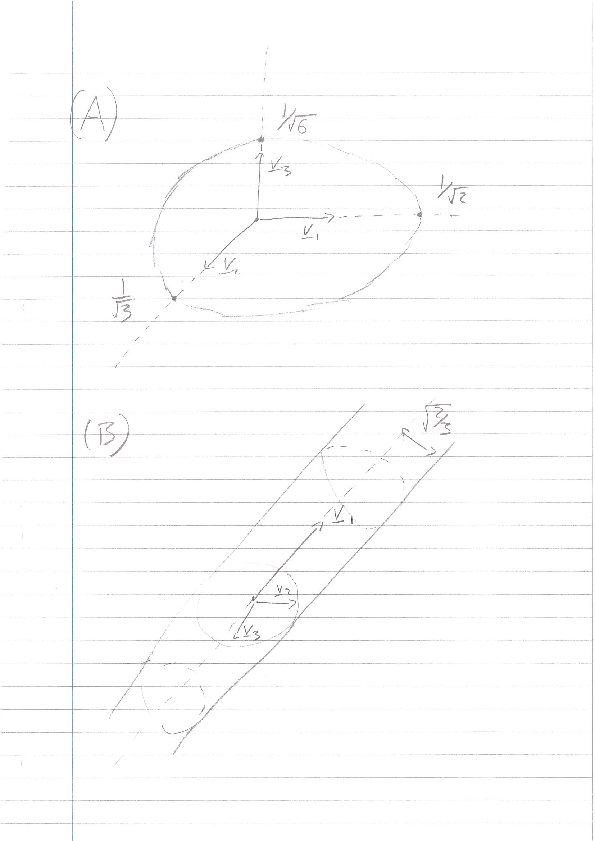
\includepdf[pages=-]{q10_diagram.pdf} \label{diag_q10}
 \item
  We will try to write \(2x^2 + 2xy + 4yz + z^2\)
  as \(\tran{\vec x} \mat A \vec x\) where \(\mat A\) is symmetric.

  Letting \(\mat A\) take its most general form, we get
  \begin{align*}
   \begin{pmatrix} x & y & z \end{pmatrix}
   \begin{pmatrix}
    a & b & c \\
    b & d & e \\
    c & e & f
   \end{pmatrix}
   \begin{pmatrix} x \\ y \\ z \end{pmatrix}
   &=
   \begin{pmatrix} x & y & z \end{pmatrix}
   \begin{pmatrix}
    ax + by + cz \\
    bx + dy + ez \\
    cx + ey + fz
   \end{pmatrix} \\
   &= ax^2 + bxy + cxz + bxy + dy^2 + eyz + cxz + eyz + fz^2 \\
   &= ax^2 + dy^2 + fz^2 + 2bxy + 2cxz + 2eyz
  \end{align*}
  so we have no choice but to let
  \(a = 2\), \(d = 0\), \(f = 1\), \(b = 1\), \(c = 0\), \(e = 2\).

  Now we can find the eigenvalues of \(\mat A\):
  \begin{align*}
   \chi_{\mat A}(t)
   &= \det(\mat A - t\mat I) \\
   &=
   \begin{vmatrix}
    2 - t & 1 & 0 \\
    1 & -t & 2 \\
    0 & 2 & 1 - t
   \end{vmatrix} \\
   &= -t(t - 2)(t - 1) + 4(t - 2) + (t - 1) \\
   &= -t(t - 2)(t - 1) + 4(t - 2) + (t - 1) \\
   &= -(t^3 - 3t^2 + 2t) + 5t - 9 \\
   &= -(t^3 - 3t^2 - 3t + 9) \\
   &= -(t^2(t - 3) - 3(t - 3)) \\
   &= -(t^2 - 3)(t - 3)
  \end{align*}
  so \(\mat A\) has eigenvalues \(3\) and \(\pm \sqrt 3\). Then the original
  surface can be written as
  \(3u^2 + \sqrt 3 v^2 - \sqrt 3 w^2 = 1\) where \(u, v, w\) are the components
  along the principle axes of this quadratic form, which are along the
  (orthogonal) eigenvectors of \(\mat A\).

  The minimum distance to the origin is then achieved when \(u^2 = \frac 13\),
  and \(v = w = 0\) so the minimum distance is \(\frac 13 \sqrt 3\).
 \item
  We have
  \begin{align*}
   \herm{(\mat A + i\mat S)}
   &= \herm{\mat A} + \herm{(i \mat S)} \\
   &= \tran{\mat A} + \conj i \tran{\mat S} \\
   &= -\mat A - i \mat S \\
   &= -(\mat A + i \mat S)
  \end{align*}
  since the hermitian conjugate of a real matrix is just its transpose.
  Therefore \(\mat A + i\mat S\) is indeed anti-hermitian.

  Then since \(\mat A + i\mat S\) is anti-hermitian,
  its eigenvalues are purely imaginary, and since \(1\) is not purely imaginary,
  \(1\) cannot satisfy its characteristic equation, and
  \(\det(\mat A + i \mat S - \mat I) \ne 0\), and particularly,
  \(\mat A + i \mat S - \mat I\) is invertible.

  If \(\mat U = (\mat I + \mat A + i \mat S)(\mat I - \mat A - i\mat S)^{-1}\),
  then
  \begin{align*}
   \mat U \herm{\mat U}
   &= (\mat I + \mat A + i \mat S)
      (\mat I - \mat A - i\mat S)^{-1}
      \herm{[(\mat I + \mat A + i \mat S)
      (\mat I - \mat A - i\mat S)^{-1}]} \\
   &= (\mat I + \mat A + i \mat S)
      (\mat I - \mat A - i\mat S)^{-1}
      [\herm{(\mat I - \mat A - i\mat S)}]^{-1}
      \herm{(\mat I + \mat A + i \mat S)} \\
   &= (\mat I + \mat A + i \mat S)
      (\mat I - \mat A - i\mat S)^{-1}
      (\mat I + \mat A + i\mat S)^{-1}
      (\mat I - \mat A - i \mat S) \\
   &= (\mat I + \mat A + i \mat S)
      (\mat I + \mat A + i\mat S)^{-1}
      (\mat I - \mat A - i\mat S)^{-1}
      (\mat I - \mat A - i \mat S) \\
   &= \mat I
  \end{align*}
  since matrices of the form \(\mat I + \mat M\) and \(\mat I - \mat M\)
  commute (either product is just \(\mat I - \mat M^2\)), and hence so do their
  inverses. So indeed \(\mat U\) is unitary.

  If \(\mat S = \begin{psmallmatrix} 1 & 1 \\ 1 & 1 \end{psmallmatrix}\) and
  \(\mat A = \begin{psmallmatrix*}[r] 0 & 1 \\ -1 & 0 \end{psmallmatrix*}\),
  then
  \begin{align*}
   \mat U
   &= \bracks*{
    \mat I
    + \begin{pmatrix*}[r]
     0 & 1 \\
     -1 & 0
    \end{pmatrix*}
    + i\begin{pmatrix}
     1 & 1 \\
     1 & 1
    \end{pmatrix}
   }
   \bracks*{
    \mat I
    - \begin{pmatrix*}[r]
     0 & 1 \\
     -1 & 0
    \end{pmatrix*}
    - i\begin{pmatrix}
     1 & 1 \\
     1 & 1
    \end{pmatrix}
   }^{-1} \\
   &=
   \begin{pmatrix*}[r]
    1 + i & 1 + i \\
    -1 + i & 1 + i
   \end{pmatrix*}
   \begin{pmatrix*}[r]
    1 - i & -1 - i \\
    1 - i & 1 - i
   \end{pmatrix*}^{-1} \\
   &=
   \frac 1{(1 - i)^2 + (1 + i)(1 - i)}
   \begin{pmatrix*}[r]
    1 + i & 1 + i \\
    -1 + i & 1 + i
   \end{pmatrix*}
   \begin{pmatrix*}[r]
    1 - i & 1 + i \\
    -1 + i & 1 - i
   \end{pmatrix*} \\
   &=
   \frac 1{2 - 2i}
   \begin{pmatrix}
    (1 + i)(1 - i) + (1 + i)(-1 + i) & (1 + i)^2 + (1 + i)(1 - i) \\
    (-1 + i)(1 - i) + (1 + i)(-1 + i) & (-1 + i)(1 + i) + (1 + i)(1 - i)
   \end{pmatrix} \\
   &=
   \frac 1{2 - 2i}
   \begin{pmatrix}
    0 & 2i + 2 \\
    2i - 2 & 0
   \end{pmatrix} \\
   &=
   \begin{pmatrix}
    0 & i \\
    -1 & 0
   \end{pmatrix}
  \end{align*}
  Then \(\chi_{\mat U}(t) = t^2 + i\), and the solutions to the characteristic
  equation (eigenvalues) are the square roots of \(-i\),
  \(\pm \frac 12 \sqrt 2(1 - i)\).
 \end{enumerate}
\end{document}
